
\documentclass{beamer}

%\setbeamertemplate{navigation symbols}{}
%\usepackage[utf8x]{inputenc}
%\usepackage{default}
\usepackage{tikz}
\usepackage{fancybox}
\usepackage{graphicx}
\usepackage{color}
%\usepackage[curves]{struktex}
\usepackage[ruled]{algorithm}
\usepackage{algorithmic}
%\usepackage{sansmathaccent}
%\usepackage{bbding}
\usepackage{pifont}
\usepackage{epstopdf}
\usepackage{multirow}

\definecolor{DarkSlateGray}{rgb}{0.184314,0.309804,0.309804}

%Mathbb
\newcommand{\R}{\mathbb{R}}
\newcommand{\N}{\mathbb{N}}
\newcommand{\C}{\mathbb{C}}

\DeclareMathOperator*{\argmin}{\arg\!\min}
\DeclareMathOperator{\spann}{span}

\newcounter{saveenumi}
\newcommand{\seti}{\setcounter{saveenumi}{\value{enumi}}}
\newcommand{\conti}{\setcounter{enumi}{\value{saveenumi}}}

%Matrix Alignment
\makeatletter
\renewcommand*\env@matrix[1][c]{\hskip -\arraycolsep
\let\@ifnextchar\new@ifnextchar
\array{*\c@MaxMatrixCols #1}}
\makeatother


\mode<presentation>
{\usetheme{boadilla} % This theme will be changed into the TUDelft lay-out
 \setbeamercovered{transparent}}
\definecolor{tudblue}{rgb}{.004,.50,.78} % definition TUDelft blue color
\definecolor{tudlightblue}{rgb}{.004,.70,.98}
\setbeamercolor{structure}{fg=tudblue}
\setbeamercolor{palette primary}{fg=white,bg=tudblue!85}       % Right field
\setbeamercolor{palette secondary}{fg=white,bg=tudblue!85}     % Middle field
\setbeamercolor{palette tertiary}{fg=tudblue!85,bg=tudblue!85} % Left field
\setbeamersize{text margin left=1cm}
\setbeamersize{text margin right=1cm}

\setbeamersize{sidebar width left=0.5cm}
\title{\bf Student Krylov Day 2015}
\date[]{February 2, 2015}
\tikzset{textlabel/.style={color=white}}
\begin{document}
\setbeamertemplate{sidebar left}  % tudblue square left above
{\vfill
\rlap{%\hskip0.1cm

\includegraphics[scale=0.33]{TUDelft/beamer-tudelft-bies.jpg} }
\vskip-5pt}
% \maketitle
\begin{frame}
 \begin{center}
  {\large \color{tudblue}\textbf{Student Krylov Day 2015}}\\
  \vspace{1cm}
  February 2, 2015
 \end{center}
\begin{tikzpicture}[overlay]
 \node at (1,-1) [rotate=10] {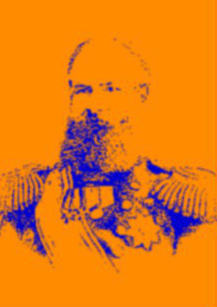
\includegraphics[width=.18\textwidth]{pics/wkrylov1.png}};
 \node at (2.5,-1.5) [rotate=-2] {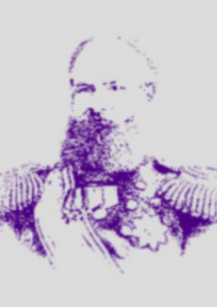
\includegraphics[width=.18\textwidth]{pics/wkrylov4.png}};
 \node at (4,-1) [rotate=15] {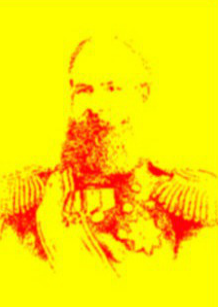
\includegraphics[width=.18\textwidth]{pics/wkrylov3.png}};
 
 \node at (9,0) [rotate=-5]{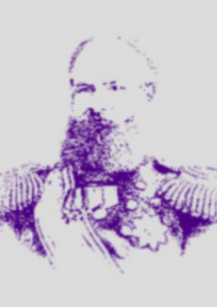
\includegraphics[width=.18\textwidth]{pics/wkrylov4.png}};
 
 \node at (0.3,3) [rotate=15]{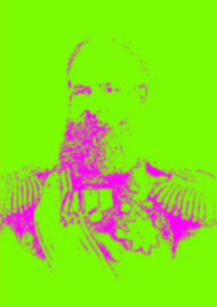
\includegraphics[width=.18\textwidth]{pics/wkrylov2.png}};
 \node at (1,3) [rotate=-5]{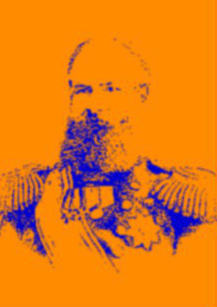
\includegraphics[width=.18\textwidth]{pics/wkrylov1.png}};

\end{tikzpicture}
\end{frame}

\begin{frame}
 \frametitle{SIAM Student Chapter at TU Delft}
 \begin{itemize}
  \item Since 2014, $\sim \! 50$ members
  \item ba{\color{red}NaN}a talks, monthly seminars, BBQ, ...
  \item Twitter: \texttt{\@SSC\_Delft}
  \item Website: \href{http://sscdelft.github.io/}{http://sscdelft.github.io/}
 \end{itemize}

   \begin{figure}[h]
  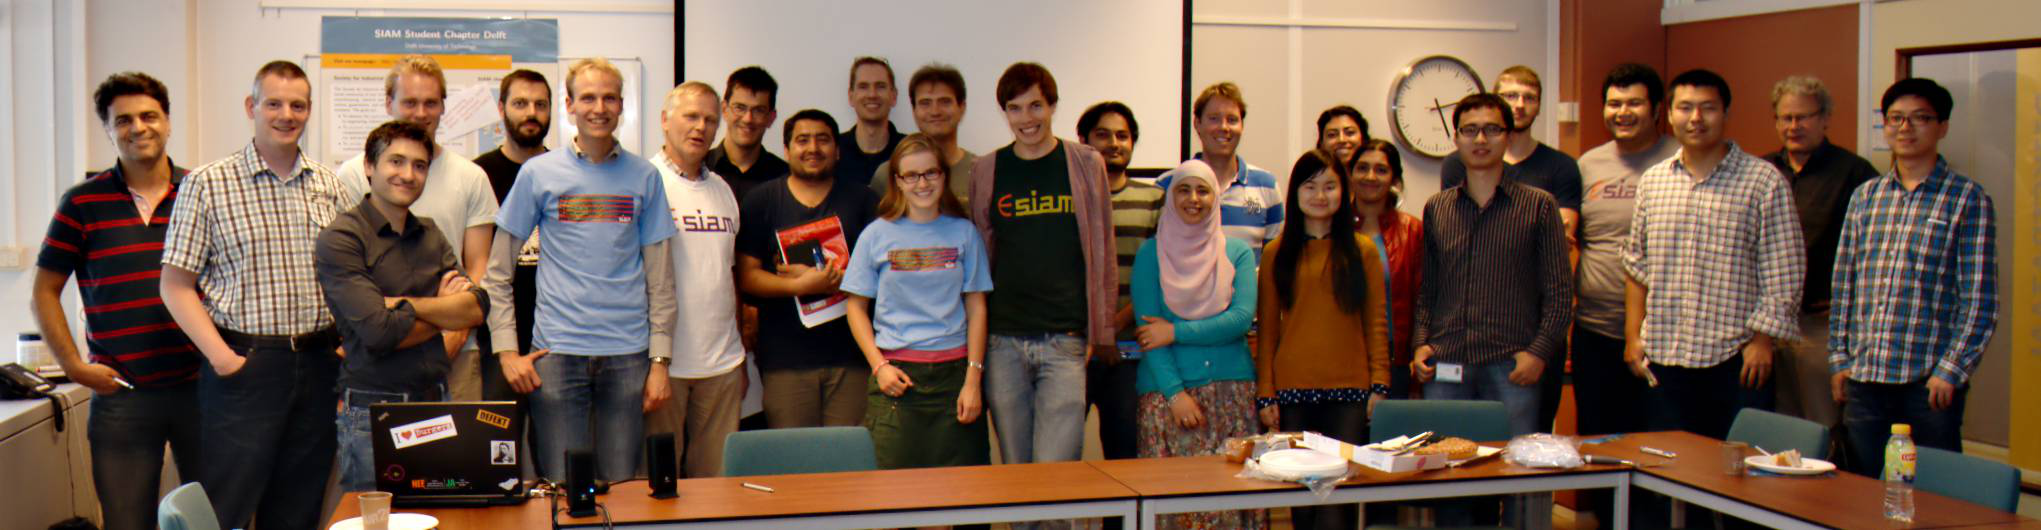
\includegraphics[width=\textwidth]{pics/ssc_delft.png}
  \end{figure}
\end{frame}


\begin{frame}
\frametitle{KD15 - Why today?}
 \begin{columns}
 \begin{column}{0.6\textwidth}
 \begin{itemize}
  \item Cornelius Lanczos was born on February 2, 1893
  \item Lanczos method
  \item Quote: \textit{``To obtain a solution in very few steps means nearly always that one has found a way that does justice to the inner nature of the problem.''}
  \pause
  \item \href{http://guettel.com/lanczos/}{{\color{red} Interesting videos!}}
 \end{itemize}

 \end{column}

 \begin{column}{0.4\textwidth}
  \begin{figure}[t]
  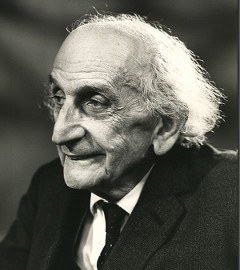
\includegraphics[width=0.7\textwidth]{pics/Lanczos240.jpg}
  \end{figure}
 \end{column}
 \end{columns}
\end{frame}

\begin{frame}
\frametitle{Today's program}
\vspace{-0.2cm}
\tiny
\begin{table}[h]
\begin{tabular}{lll}
10:10 - 10:50 & P. Sonneveld & IDR-CGS-BiCGSTAB-IDR(s) - a case of serendipity -\\ [0.5ex]
\hline \\ [-1.5ex]
11:00 - 11:20 & Manuel & Krylov methods for shifted linear systems \\ [0.5ex]
11:20 - 11:40 & Xian-Ming & Recent progresses in Krylov subspace methods\\ 
                        & & for solving complex symmetric linear systems\\  [0.5ex]
11:40 - 12:00 & Ian & Krylov and Matrix Balancing for fast Field \\ 
              &     & of Value Type Inclusion Regions\\  [0.5ex]
% & & \hfill \tiny{Chairman: Reinaldo }  \\
\hline \\ [-1.5ex]
12:00 - 13:30 & & Lunch at TU Delft Sports Center \\ [0.5ex]
\hline \\ [-1.5ex]
13:30 - 13:50 & Heiko & Preconditioning of Large-Scale Saddle Point \\
                    & & Systems for Coupled Flow Problems\\ [0.5ex]
13:50 - 14:10 &J\"orn & A Krylov Subspace Approach to Modeling of \\
                     & & Wave Propagation in Open Domains\\ [0.5ex]
14:10 - 14:30 & Jing & A conjugate gradient based method for \\
                   & & frictional contact problems\\ [0.5ex]
% & & \hfill \tiny{Chairman: Tom{\'a}{\v s}} \\
\hline \\ [-1.5ex]
15:00 - 15:20 & Tom{\'a}{\v s} & On the numerical behaviour of the CG method\\ [0.5ex]
15:20 - 15:40 & Patrick & Krylov subspace methods for matrix equations \\
                  & & which include matrix functions\\ [0.5ex]
15:40 - 16:00 & Ana & On Low-rank Updates of Matrix Functions\\ [0.5ex]
% & & \hfill \tiny{Chairman: Heiko}  \\
\hline \\ [-1.5ex]
16:30 - 16:50 & Reinaldo & Induced Dimension Reduction method \\
            & & to solve the Quadratic Eigenvalue Problem \\ [0.5ex]
16:50 - 17:10 & Mario & Rational Least Squares Fitting using Krylov Spaces\\ [0.5ex]
17:10 - 17:30 & Sarah & Probabilistic bounds for the matrix condition  \\
                    & & number with extended Lanczos bidiagonalization\\ [0.5ex]
% & & \hfill \tiny{Chairman: Manuel}\\
\hline \\ [-1.5ex]
% 17:00 - 18:00 & & Snacks \& drinks at TU Delft
\end{tabular}
\end{table}
\end{frame}

\begin{frame}
 \frametitle{Today's program - Some things to notice!}
 \begin{columns}
 \begin{column}{0.6\textwidth}
 \begin{itemize}
  \item Talks are {\color{tudblue}15+5 mins}
  \item {\color{tudblue}Lunch} at TU Delft Sports Center (walking distance)
  \item {\color{tudblue}Coffee} machines work with \textit{TU Delft} cards
  \item 19:00 - Reservation at {\color{tudblue}San Marco} (Brabantse Turfmarkt 23, 2611 CL Delft)
 \end{itemize}

 \end{column}

 \begin{column}{0.4\textwidth}
  \begin{figure}[t]
  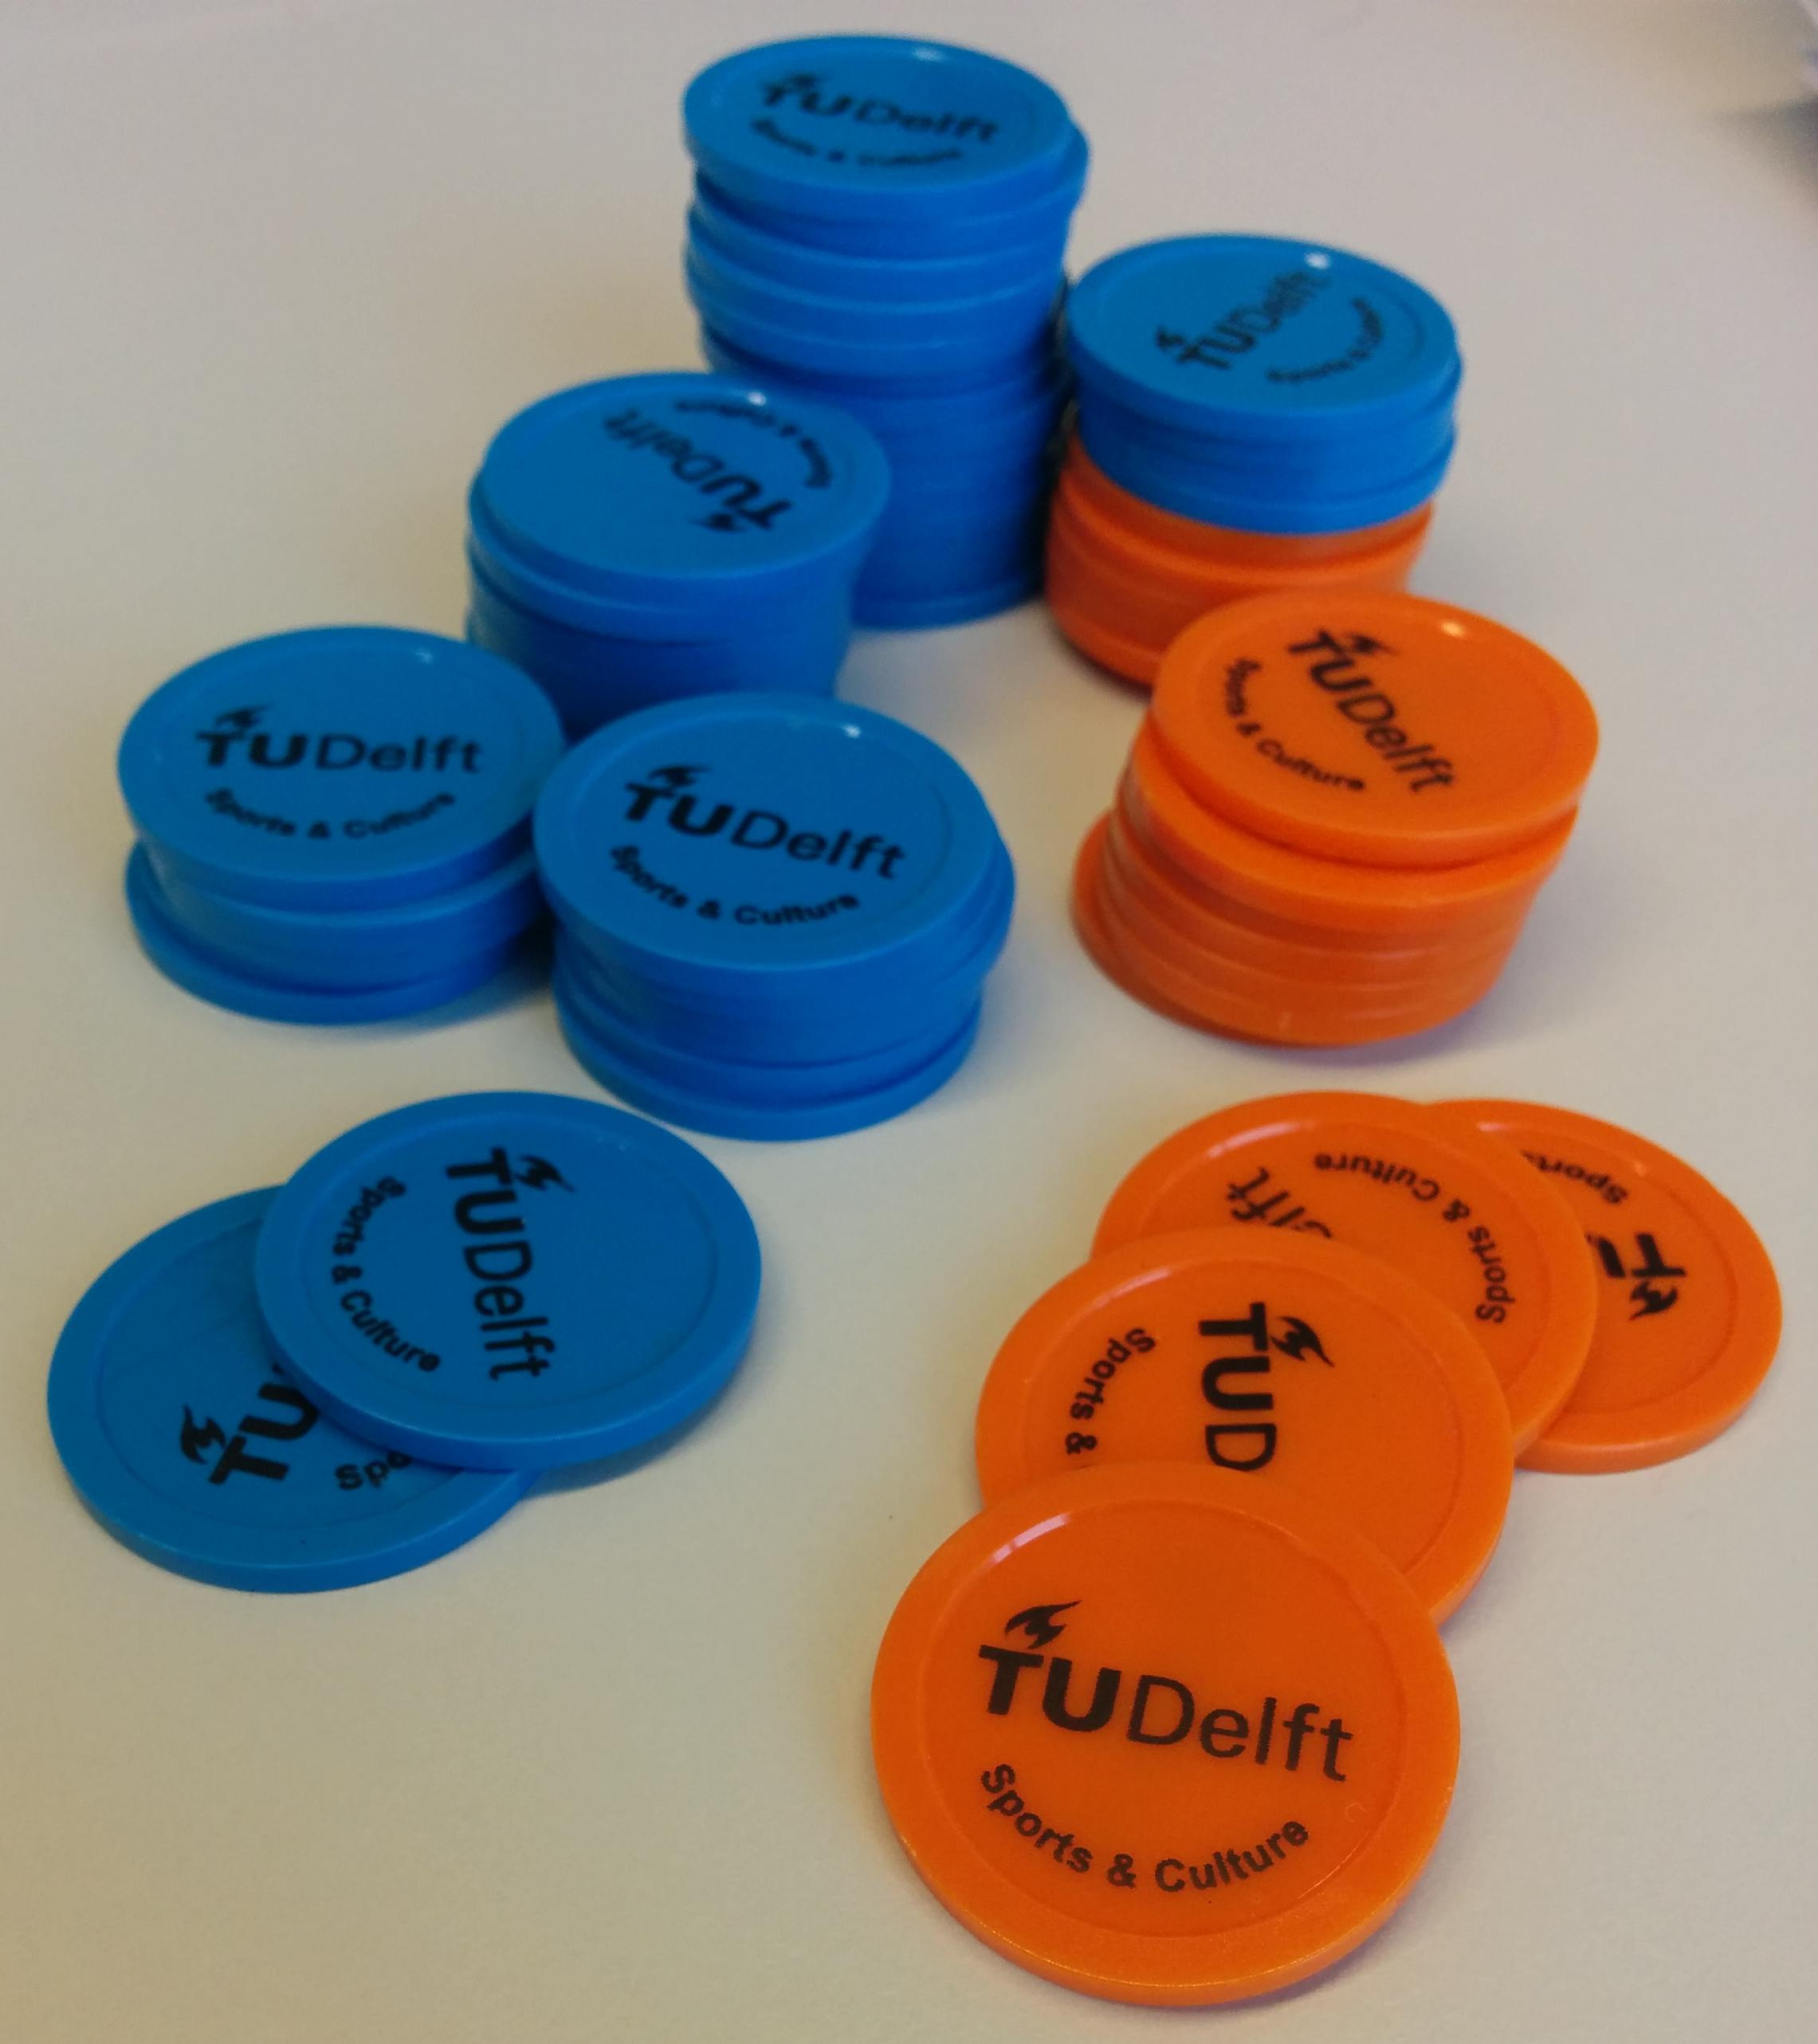
\includegraphics[width=0.7\textwidth]{pics/money.jpg}\\ \vspace{0.6cm}
  
\includegraphics[width=0.7\textwidth]{pics/sanmarco_logo.png}
  \end{figure}
 \end{column}
 \end{columns}
\end{frame}

\begin{frame}
\huge{
  \begin{figure}[t]
  
\includegraphics[width=0.5\textwidth]{pics/twitter-logo.png}
  \end{figure}
 \center{
Please use the designated hashtag \texttt{\#KD15}
}
}
\end{frame}

\begin{frame}
\frametitle{Let's welcome Peter Sonneveld}
 \begin{columns}
 \begin{column}{0.6\textwidth}
 Peter's work has huge impact on research in Krylov methods.
 \begin{itemize}
  \item IDR [1980]
  \item CGS [1989]
  \item IDR($s$) [2008]
 \end{itemize}
 \end{column}

 \begin{column}{0.4\textwidth}
  \begin{figure}[t]
  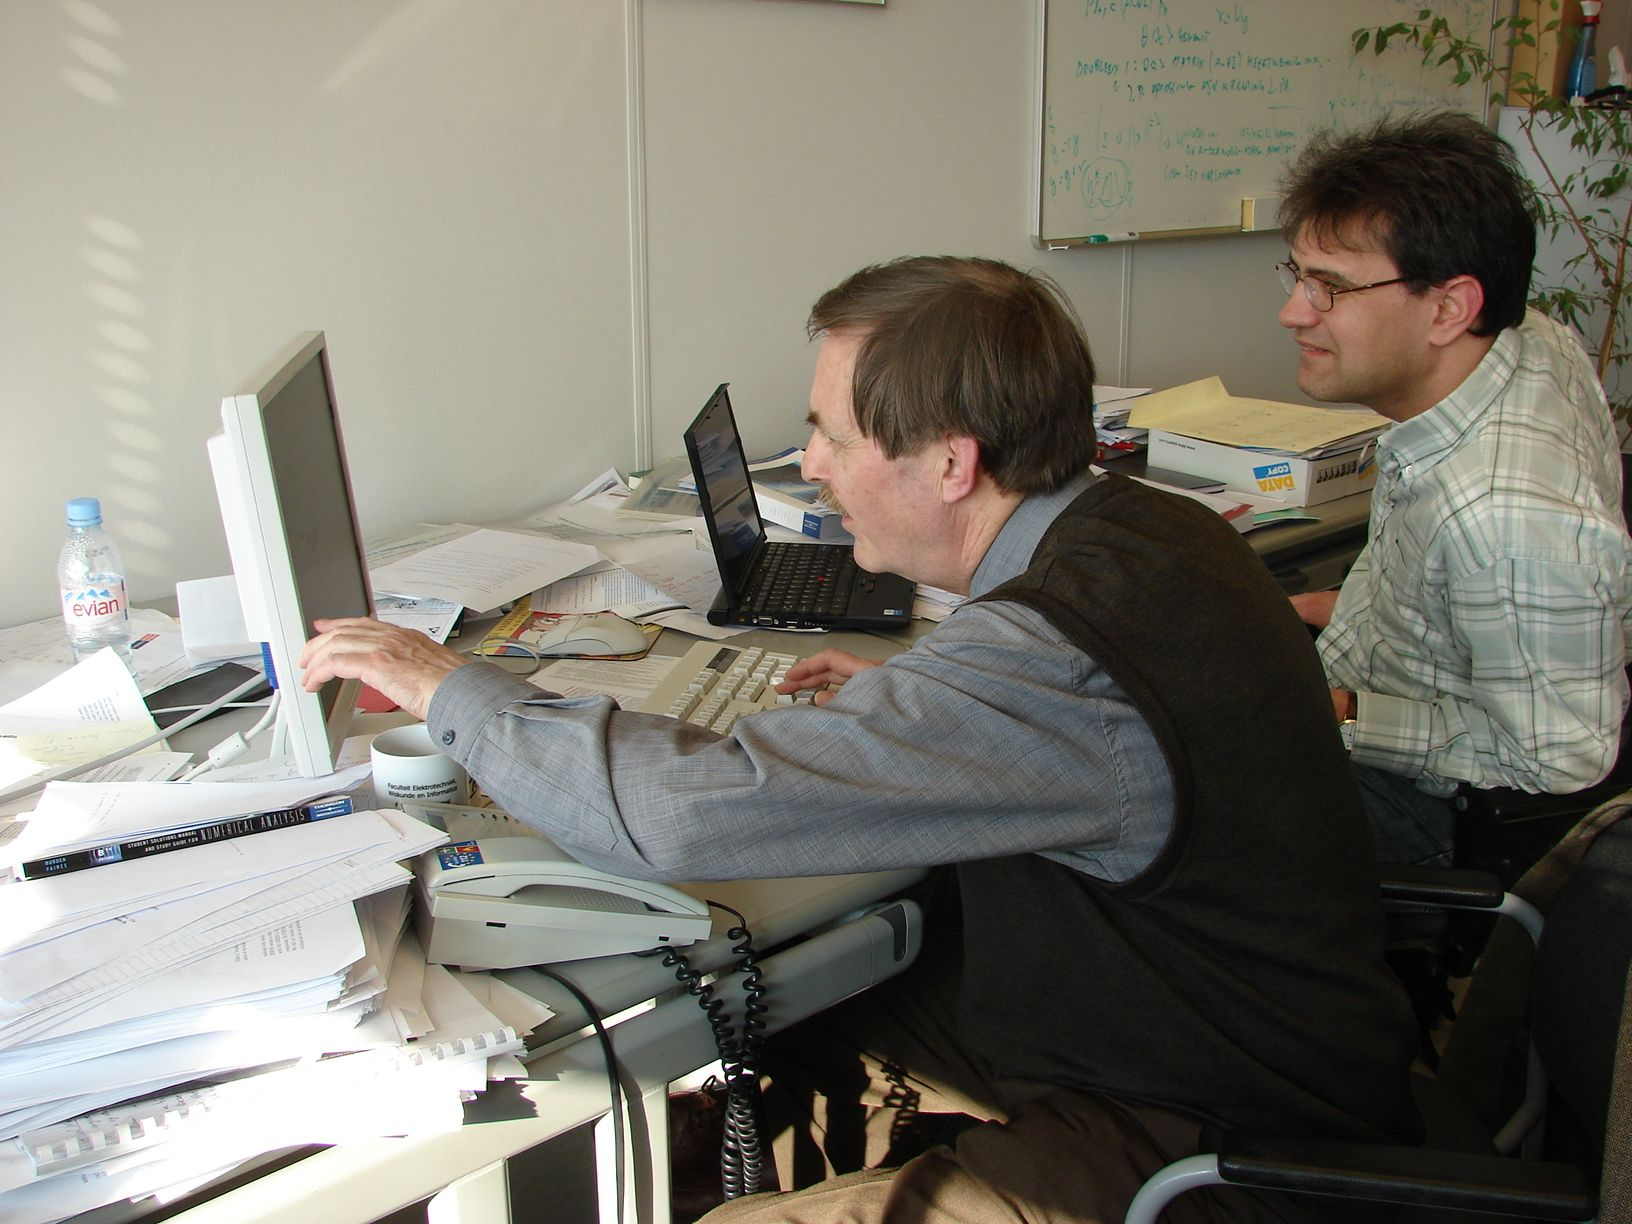
\includegraphics[width=0.9\textwidth]{pics/idr1.jpg}
  \end{figure}
 \end{column}
 \end{columns}
 \vspace{1cm}
 \pause
 \begin{center}
  \textit{Have a nice day!}
 \end{center}
\end{frame}

\begin{frame}
 \frametitle{Group picture}
   \begin{figure}[t]
   \vspace{-0.3cm}
  
\includegraphics[width=0.7\textwidth]{pics/baustelle.png}
  \end{figure}
\end{frame}

\begin{frame}
 \frametitle{In the future...}
 \begin{itemize}
  \item In the \href{http://www.sanmarco.nl/}{near future}:
    \begin{figure}[t]
  
\includegraphics[width=0.6\textwidth]{pics/sanmarco_logo.png}
  \end{figure}
  \pause
  \vspace{0.3cm}
  \item Future meetings:
  \begin{itemize}
  \item SIAM Conference on Applied Linear Algebra (LA15).
  \item Student Chapter Manchester (Mario)
  \item Student Chapter Magdeburg (Heiko, Patrick)
  \item Student Chapter Prague (Tom{\'a}{\v s})
  \end{itemize}
  \pause
  \item {\color{red}Krylov Day 2016} \texttt{\#KD16}
 \end{itemize}

\end{frame}


\end{document}
